\section{Finite State Machines}
\label{sec:finite_state_machines}

Finite state machines (FSMs) are a powerful method of modelling systems whose output depends on the entire history of their inputs (as opposed to memoryless systems, where the output depends on the current input only).
FSMs are widely used in various fields, including computer science, control systems, and digital circuit design. They can be classified into two main classes: deterministic finite state machines (DFSMs) and non-deterministic finite state machines (NDFSMs).

Mathematically, a finite state machine is defined as a 6-tuple $(S, I, O, \delta, \lambda, s_0)$, where:

\begin{itemize}
    \item $S$ is a finite set of states.
    \item $I$ is a finite set of input symbols (input alphabet).
    \item $O$ is a finite set of output symbols (output alphabet).
    \item $\delta: S \times I \to S$ is the state transition function, which maps a state and an input symbol to the next state.
    \item $\lambda: S \times I \to O$ is the output function, which maps a state and an input symbol to an output symbol.
    \item $s_0 \in S$ is the initial state.
\end{itemize}

The FSM processes a sequence of input symbols, transitioning between states according to the state transition function $\delta$ and producing output symbols according to the output function $\lambda$.
The behavior of an FSM can be represented using state transition diagrams or state transition tables.



\subsection{Turnstile FSM}
\label{subsec:turnstile_fsm}

As an example, we consider a turnstile that allows entry when a coin is inserted and locks when a person pushes through.
The FSM for this turnstile can be represented by the state transition diagram in Figure \ref{fig:fsm_turnstile_diagram} \cite{wiki:turnstile_fsm} and the state transition table in Table \ref{tab:fsm_turnstile_table} \cite{wiki:turnstile_fsm}.

\begin{figure}[H]
    \centering
    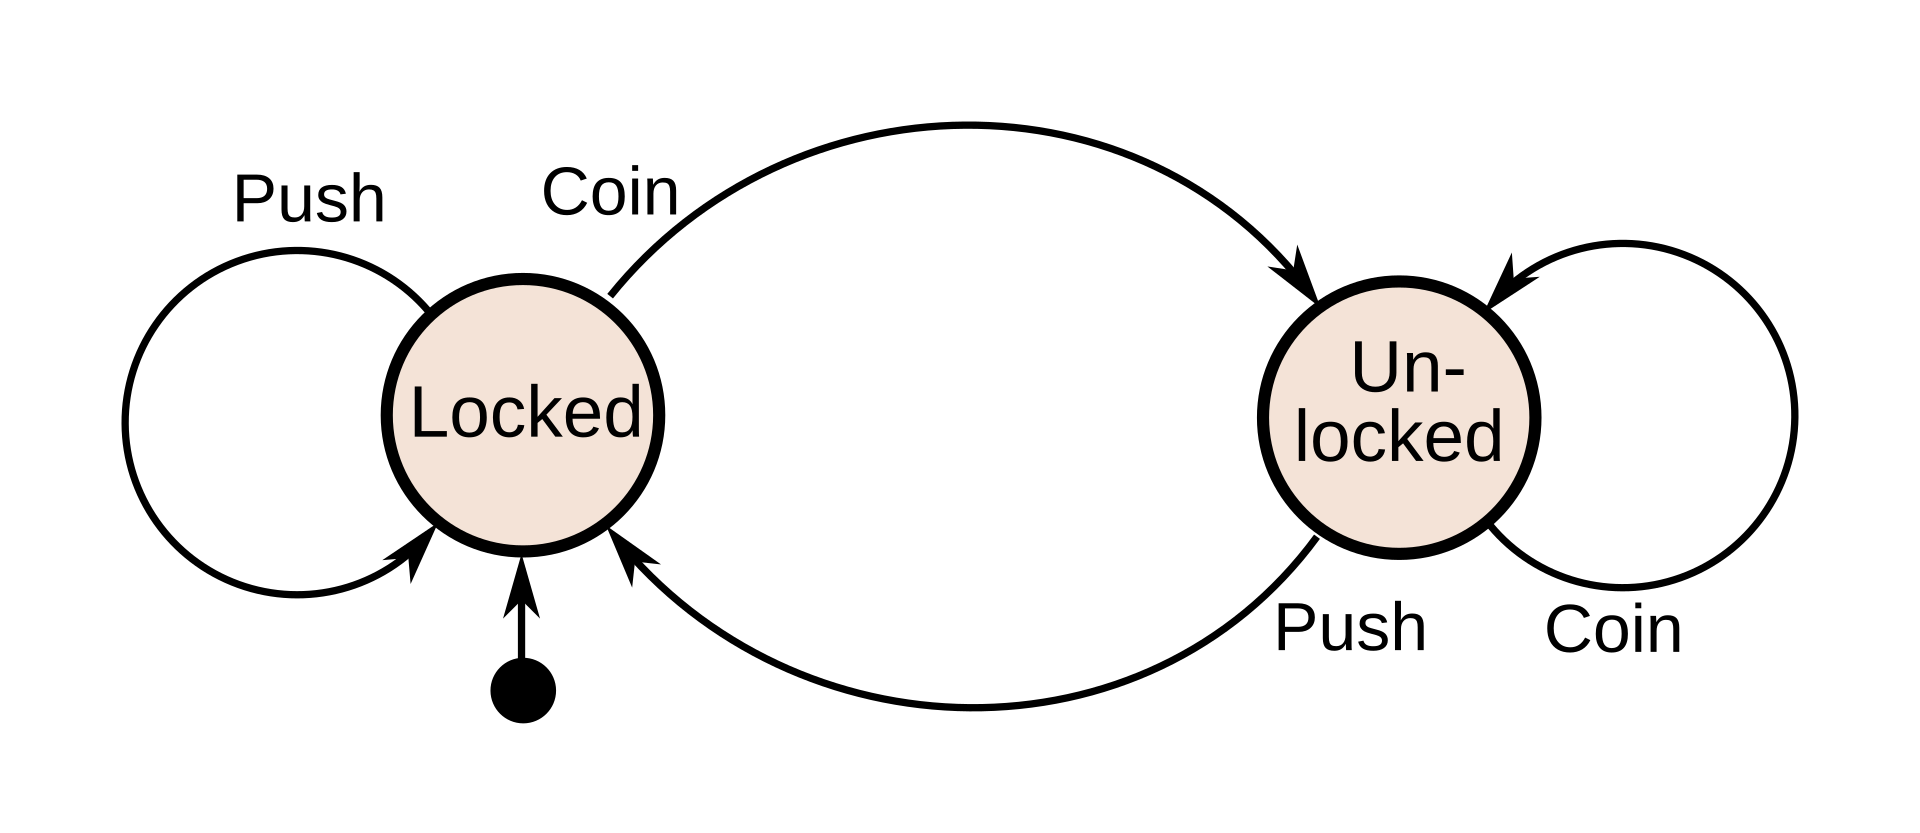
\includegraphics[width=0.7\textwidth]{img/fsm_turnstile.png}
    \caption{Turnstile FSM State Transition Diagram}
    \label{fig:fsm_turnstile_diagram}
\end{figure}

\begin{table}[H]
    \centering
    \begin{tabular}{|c|c|c|l|}
        \hline
        \textbf{Current State}    & \textbf{Input} & \textbf{Next State} & \textbf{Output}                                             \\
        \hline
        \multirow{2}{*}{Locked}   & Coin           & Unlocked            & Unlocks the turnstile so that the customer can push through \\
                                  & Push           & Locked              & None                                                        \\
        \hline
        \multirow{2}{*}{Unlocked} & Coin           & Unlocked            & None                                                        \\
                                  & Push           & Locked              & When the customer has pushed through, locks the turnstile   \\
        \hline
    \end{tabular}
    \caption{Turnstile FSM Transition Table}
    \label{tab:fsm_turnstile_table}
\end{table}

The FSM starts in the \textit{Locked} state.
When a coin is inserted, it transitions to the \textit{Unlocked} state and allows the customer to push through.
If the customer pushes through while in the \textit{Unlocked} state, the FSM transitions back to the \textit{Locked} state.
If a coin is inserted while in the \textit{Unlocked} state, the FSM remains in the same state.

